
\graphicspath{  {mainmatter/Lyons_2003/} }
\title*{2003: Designing, Playing, and Performing with a Vision-based Mouth Interface}
\titlerunning{A Vision-based Mouth Interface}

\author{Michael J. Lyons, Michael H{\"a}hnel, and Nobuji Tetsutani}
\authorrunning{Lyons et al.}

%\institute{Michael J. Lyons \at Ritsumeikan University, Kyoto, Japan, \email{michael.lyons@gmail.com}}
%\and Name of Second Author \at Name, Address of Institute \email{name@email.address}}
%
%
\maketitle



\abstract*{The role of the face and mouth in speech production as well as non-verbal communication suggests the use of facial action to control musical sound. Here we document work on the Mouthesizer, a system which uses a headworn miniature camera and computer vision algorithm to extract shape parameters from the mouth opening and output these as MIDI control changes. We report our experiences with various gesture-to-sound mappings and musical applications, and describe a live performance which used the Mouthesizer interface.}

% \cite{}
\section{Introduction}
%\label{lyons-sec:1}
Articles on new interfaces for computer music often begin with a call for greater embodiment in the way computers are operated. This claim is sometimes backed up by citing developments in cognitive science which stress the importance of physical and physiological context for understanding the mind \cite{Varela:1992}. Similar considerations may be applied in the domain of   machine-mediated human interaction. Current ways of interacting with computers neglect most of the physiology of human-human interaction and are surely unsuitable for most forms of communication, especially expressive forms such as music.

Working at McGill University half a century ago, Wilder Penfield and his colleagues \cite{Penfield:1950} mapped the sensory-motor cortex by electrical stimulation of conscious patients undergoing neurosurgery. Their pictorial summary of the findings, the somatosensory and motor homunculi, are widely known and their importance for human-machine interaction \cite{Card:1991}as well as musical interfaces \cite{Gillespie:1999} has been recognized. A striking aspect of the motor homunculus (Figure~\ref{lyons-fig:1}) is the relatively large area devoted to the organs critical for verbal and non-verbal human communication: the lips, mouth, tongue, larynx, and the face.

\begin{figure}[t]
\centering
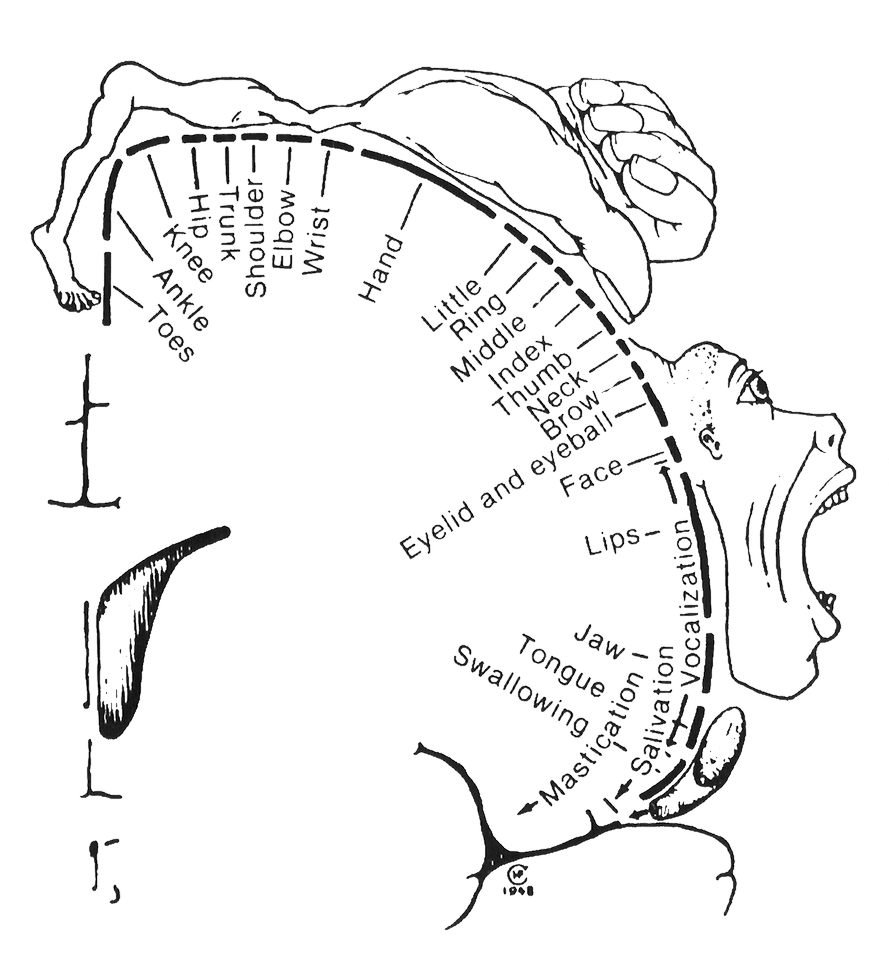
\includegraphics[width=90mm]{lyons_fig1}
\caption{The motor homunculus or representation of body areas in the motor cortex \cite{Penfield:1950}.}
\label{lyons-fig:1} 
\end{figure}

The importance of the face and especially the mouth in communication inspired us to develop a musical controller which takes input from facial actions. The face, especially the mouth area, is involved both in sound production, in speech, singing, and in non-verbal emotional communication, in facial expression. It therefore seemed interesting to attempt to design a musical interface making use of our expertise for muscular action of the face.

This paper reports work using a video-based approach and focuses on the area of the mouth.  Preliminary results of the study were previously published as a short paper \cite{Lyons:2001}. The current article is intended as a more complete record of the project in which we: (a) state the context of the work by reviewing related studies (section 2); (b) describe the implementation in detail including more recent developments, discussing design considerations as well as lessons learned (section 3); (c) report our experience with several mappings and musical applications of the controller (section 4); and (e) describe a public performance in which the controller was used (section 5); and (f) conclude with general observations (section 6).

\section{Related Work}
%\label{lyons-sec:2}

\subsection{Mouth and Vocal Tract Controllers}
%\label{lyons-subsec:1}

The fact that oral cavity shape influences the human voice means there are complex neural circuits relating for muscular control the mapping of shape to sound effect. Use of the oral cavity for modulating sounds other than those produced by the vocal tract is probably as old as instrumental music itself, evidenced by the presence of instruments like the mouthbow in folk cultures around the world. 

Functioning by the same principle as acoustic mouth controllers, the TalkBox, which enjoyed popularity in the 1970's, allows a player to directly filter an audio signal with the acoustic transfer of the oral cavity. Holding a small speaker in the mouth, the player modulates the signal by varying the oral cavity shape and position of the tongue. Since the actual acoustic properties of the mouth modify the signal, the TalkBox is intuitive to use. However the range of sound effects is limited by the same acoustic possibilities. It is also requires the player/singer to keep the device in their mouth.
The Vocoder \cite{Dudley:1939} allows effective vocal tract control of synthesized electronic sounds via audio signal processing extraction of voice parameters to modulate synthesized sounds. Using a Vocoder is more akin to speaking or singing than to playing an instrument since it is activated by sounds produced in the vocal tract itself.

By contrast, the interface developed by Orio \cite{Orio:1997} probes the shape of the oral cavity by stimulation with an external acoustic source. Shape parameters extracted from analysis of the response are output as MIDI controls. Orio found that users could easily learn to control two independent parameters by varying mouth shape, but greater difficulty controlling three parameters.
Vogt et al. \cite{Vogt:2002} used ultrasound imaging to measure tongue position and movement in real-time for sound synthesis control. With the Tongue ‘n' Groove, an ultrasound device is held below the jaw and an image of the tongue contour reconstructed, or alternatively, optical flow due to tongue motion is calculated. Several mapping metaphors were explored; e.g. tongue position was used to play a physical model of the singing voice.

\subsection{Vision-Based Musical Interfaces}
%\label{lyons-subsec:2}

Several previous works have used computer vision techniques for musical interaction. 

Multimedia installation artist David Rokeby has experimented for many years with his Very Nervous System,\footnote{\url{http://www.davidrokeby.com/vns.html}} or VNS, which is now available for purchase. The VNS web pages do not give an explicit description of what it computes, but VNS appears to be based primarily on pixel calculations responsive to movement, such as temporal differencing in user defined trigger zones. 

The BigEye software,\footnote{\url{http://steim.org/2012/01/bigeye-1-1-4/}} available commercially from STEIM, allows tracking of coloured objects against a set of definable regions in the video frame, with variables such as relative position, size, and speed output as MIDI parameters.

The EyesWeb software platform \cite{Camurri:2000b}, freely available from the InfoMus group at the University of Genoa, includes several computer vision modules allowing tracking of objects and coloured blobs as well as modules for estimation of affective and expressive qualities of movements, with several output options including MIDI and OSC.

Some vision-based controllers adapt software developed for non-musical purposes. The DanceSpace system \cite{Paradiso:1997d} added to the MIT Media Lab's Pfinder vision-based person tracker, to allow mapping of movements of tracked limbs, torso, and to changes in musical parameters.

The Augmented Groove system \cite{Poupyrev:2000} uses the University of Washington HIT Lab's Augmented Reality (AR) Toolkit which supports tracking of high-contrast two dimensional patterns. The AR Toolkit can extract translation, rotation, and tilt of objects labeled with the patterns. The Augmented Groove system maps tracking parameters to MIDI control changes, allowing users to modulate sequencer loops by manipulating physical objects.

Those with the resources often prefer to develop specific software for a project as this allows greater control over how the solution is implemented. 

The Iamascope's vision-to-music subsystem \cite{Fels:1999} divides the video input frame into detection zones mapped to notes of a chord. A motion detection algorithm allows note triggering with free gestures. The kaleidoscope subsystem mirrors the video input to display intriguing visual feedback of the user's own gestures. 

With the Imaginary Piano \cite{Tarabella:2000}, video input from a camera facing the player is analyzed with a motion detection algorithm which responds to movement of the hands below a vertical threshold to trigger piano notes having pitch determined by the horizontal coordinate.

Ng \cite{Ng:2002} seems to be the only other work to suggest using a vision-based interface to transform facial gestures to MIDI controls. A video demo of their prototype was shown at NIME-02, but details of their implementation have not yet been published.

\section{Design Evolution}
%\label{lyons-sec:3}
\subsection{Face Tracking System}
%\label{lyons-subsec:1}

At the outset, our aim was to utilize actions from several areas of the face for musical expression, including movements of the eye regions, eyebrows, mouth, cheeks and movements of the whole head. We started by building upon a vision-based face tracking system developed in our group at ATR.  The first prototype was implemented on an SGI O2 computer, using the O2's built-in framegrabber and the IRIS video library. This allowed acquisition of NTSC quarter-frame images (320x240 pixels) at 15 fps. This is the minimum useable frame rate for most musical applications: latencies are noticeable but still tolerable.

We initially considered using a more sophisticated feature shape representation \cite{Lyons:1999,Pantic:2000}, but experiments showed that the shadow area of the mouth could be extracted by a very simple colour and intensity thresholding algorithm. First, a region large enough to include the mouth area with certainty is chosen, based on the inter-ocular distance from the face tracking module. Next, pixels in this region satisfying  the following equation:

%
\begin{equation}
I < I_{min} \; \;  \; and \;  \;  \; R > R_{max}
%\label{lyons-eq:01}
\end{equation}
%

are segmented, where I is pixel intensity and R is its red component and $I_{min}$ and $R_{max}$ are set thresholds. With appropriate values for the thresholds, under a large region of lighting conditions most of the pixels satisfying this condition belong to the shadow area of the mouth. Segmentation by colour thresholding is widely used to track objects in vision systems. For example skin colour is used as a cue in many face detection algorithms, though it is widely known to be affected by the intensity and colour of the illumination. Thresholding of the mouth shadow area seems to be considerably more stable to such illumination changes because we are detecting the absence of a surface: the appearance of the cavity is more robust than that of the surrounding skin areas. Use of the automatic gain and colour balance control on the cameras adds to the robustness of the system to lighting changes.

The system has some limitations, for example, dark facial hair near the mouth may also be selected by the thresholding operation. With very dark skin, thresholds may need to be changed or additional lighting used.

The pixels obtained by the thresholding operation were analyzed using a principal components analysis \cite{Duda:1973} to find the major and minor axis of the segmented area, which approximates an elliptical blob. Use of an algorithm based on colour segmentation and invariant statistics of the pixel coordinates has the advantage that it is robust to translation and in plane rotation of the mouth region. Hence, movements of the camera, unavoidable due to slight vibration of the beam, do not strongly affect the shape parameters extracted from the image. Higher level algorithms based on tracking loops for position estimation, would not share this property. 

The two shape parameters were mapped to two MIDI control change values. These were used to control timbre of various physically modelled instruments using the demos Perry Cook's Synthesis ToolKit \cite{Cook:1999a} running on the same SGI O2. Segmented pixels were displayed in red on a video output of the players face. Experiments with this system quickly convinced us that the mouth functions well as a controller of synthesized sound and we next concentrated on developing a mouth controller for use in actual musical performance situations.

\subsection{Headworn System}
%\label{lyons-subsec:2}

\begin{figure}[t]
\centering
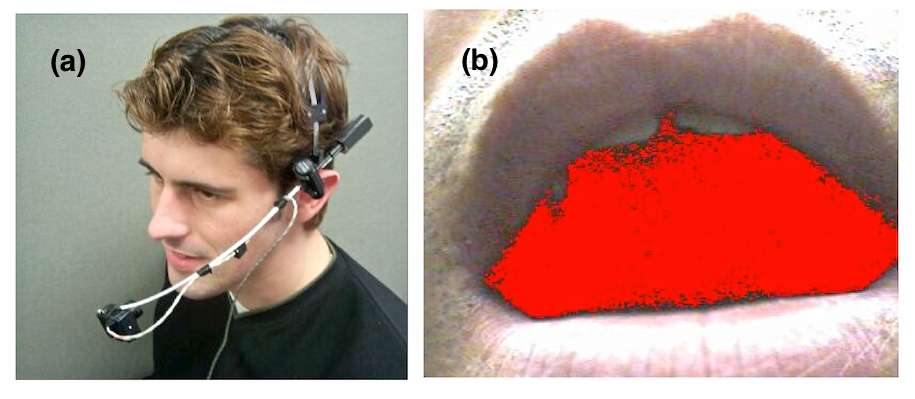
\includegraphics[width=90mm]{lyons_fig2}
\caption{(a) the headset and (b) a view from the camera}
\label{lyons-fig:2} 
\end{figure}

When we began this research, the face tracking module was limited to a video processing rate of 13 fps, and tracking was interrupted by large speed or amplitude of head movements. Tracking performance has since been increased to full frame rate, but robustness it is still not adequate for live performance situations. In addition, the apparent facial expression in 2D projection depends on head orientation \cite{Lyons:2000}. Finally, experiments with the tracking system convinced us that a wearable system would allow performers greater mobility and comfort. 

These considerations led us to concentrate research on a system based on a head mounted camera pointed directly at the mouth area (Figure~\ref{lyons-fig:2}). Camera distance and focal length of the lens were chosen so that that the input video frames contained the facial region of the mouth, and excluded other areas that are picked up by  thresholding such as the nostrils and, occasionally, a shadow below the lower lip. This eliminates the need for a face tracking system. 

The headset is a modified Shure SM10A with the microphone and beam assembly removed and replaced with a miniature video camera mounted on a homebuilt aluminum arm. It is important to counterbalance the weight of the camera. Miniature, lightweight video cameras are now widely available (Figure~\ref{lyons-fig:3}). Most of the work reported here used a Keyence CK-200B miniature colour CCD camera with standard NTSC analog output. We also tried the expensive Elmo QN42H camera pictured in the figure, which gave similar results. The Keyence camera is economical and ideally suitable for use with the Mouthesizer. 

\begin{figure}[t]
\centering
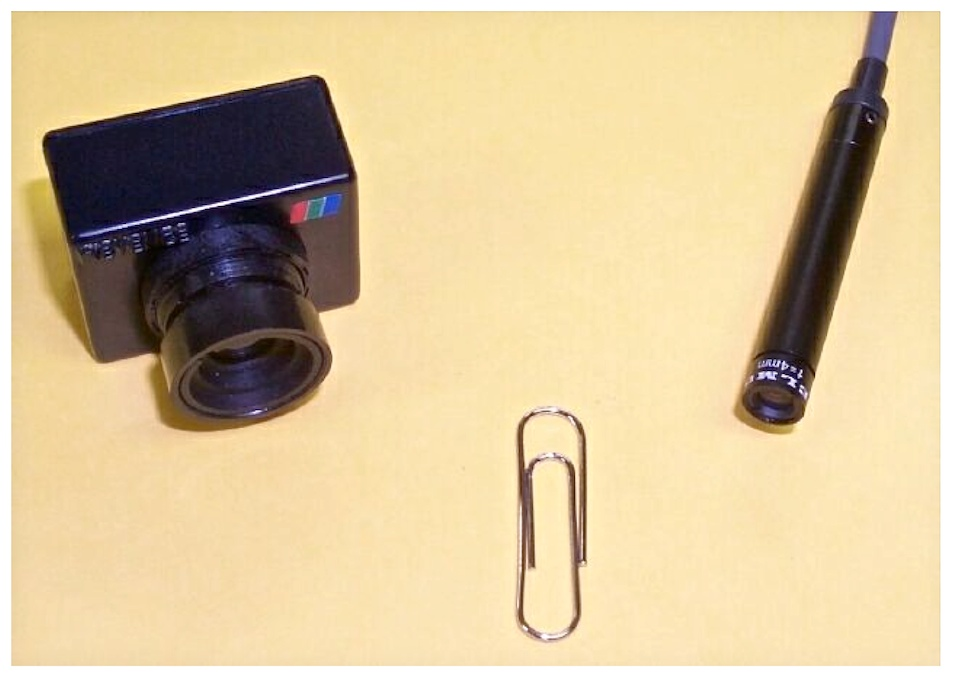
\includegraphics[width=90mm]{lyons_fig3}
\caption{Two miniature CCD cameras used in this work.}
\label{lyons-fig:3} 
\end{figure}

\subsection{Machine-Vision Board}
%\label{lyons-subsec:3}

To demonstrate the feasibility of an inexpensive, portable, and stable system we next implemented a hardware prototype. We selected the Cognachrome 2000, made by Newton Labs (Renton, WA), a dedicated machine vision board based on the Motorola 68322 processor. The Cognachrome tracks the position, size, aspect ratio, and orientation of several colour blobs at 60 Hz and a spatial resolution of 200x250 pixels, with a proprietary algorithm that uses colour and intensity thresholding and connected region analysis. Video input and output is NTSC format and data communication is via a serial port. Mouth shadow blob dimensions as detected by the board were remapped to two MIDI control changes via a program running on a desktop program. The Cognachrome is programmable allowing onboard implementation of MIDI communications. However, it has several disadvantages, the most important of which were that mouth shadow tracking was more sensitive to illumination changes than with the software algorithm we implemented and that the tracking algorithm could not be easily modified. 

\subsection{Current Implementation}
%\label{lyons-subsec:4}

Flexibility considerations led us to return to a software implementation, using Visual C++ and Direct-X running under Windows. The current Mouthesizer operates as a Direct-X filter, allowing use of the system with any input video device for which a driver is available.
Several improvements to the algorithm were made. Connected region analysis is applied after the colour and intensity thresholding operation. This removes thresholded pixels outside of the mouth shadow area. Two types of simple temporal filters were added to remove noise due to rapid fluctuations in lighting or shadows (Figure~\ref{lyons-fig:4}).

\begin{figure}[t]
\centering
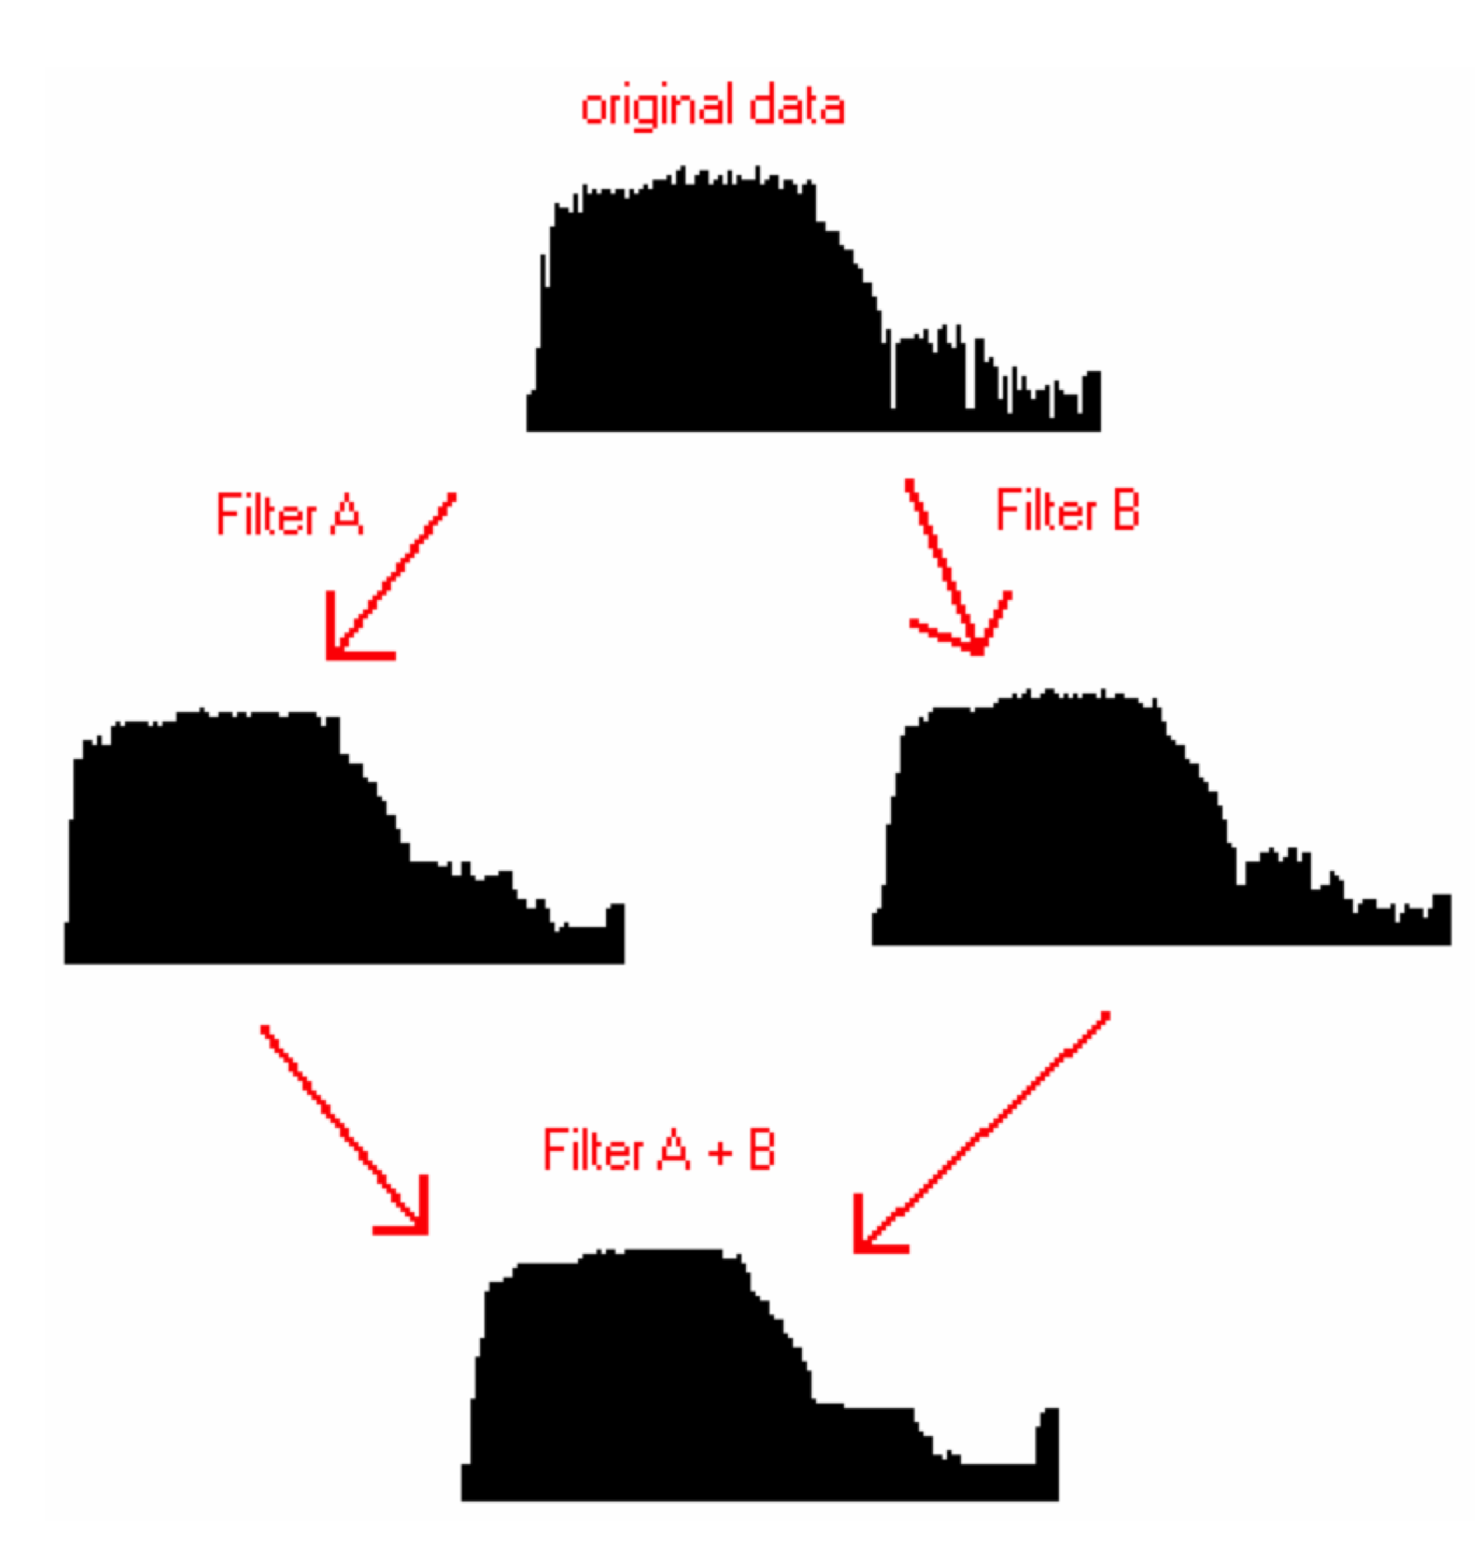
\includegraphics[width=90mm]{lyons_fig4}
\caption{Filtering feature parameters from the Mouthesizer}
\label{lyons-fig:4} 
\end{figure}

Filter A discards any output that differs from the average of the two most recent output values by more than a set threshold. 

Filter B temporally smoothes the data by averaging current outputs with previous ones. The filters can be independently turned on or off while the software is running.

A desktop system on a Pentium II with a Winnov Videum capture card ran at 30 fps, while on a Pentium III notebook with I-O Data PCCAP video capture card the system ran at 15 fps, both at a resolution of 320x240 pixels. The system now also works with Firewire and USB cameras at full frame rate. Some recent palmtops should now have sufficient processing power to run the Mouthesizer algorithm at low resolution, which would allow it to be used as a fully wearable device.

\section{Mapping and Applications}
%\label{lyons-sec:4}

Below we first report gesture-to-sound mappings which were found to work well with the Mouthesizer. Then we describe actual applications of the Mouthesizer to playing music. Most of our experiments with mappings and applications were made with the Nord Modular Virtual Analog Synthesizer (from Clavia, Sweden). With the Nord Modular, synthesis or audio effects patches are edited in software with an intuitive graphical interface, but run on dedicated DSP hardware. Patch variables were easily adjusted using control panel knobs and driven by external MIDI controllers.

\subsection{Mapping}
%\label{lyons-subsec:1}

In all cases the mouth shape parameters were mapped to two MIDI control changes. The mappings discussed below were not intended to be one-to-one mappings of shape to sound. Rather, two principles guided our experimentation: the role of the mouth as a filter in sound production and the action of the facial muscles in the facial expression of emotion. Our goal was to try to create intuitive and compelling mappings from action to sound by making use of existing motor expertise and brain maps for sound production and emotional expression. 

Musical interface mapping is a subtle issue \cite{Hunt:2003} and there is room for further exploration of the expressive potential of the Mouthesizer. For example, for some vocal consonants the lips and tongue act as sources of sound. Expression of certain emotions such as surprise or mirth can have relatively rapid onset dynamics, which may not be well modelled as continuously changing controls. Cursory experiments suggested that it should also be interesting to use the Mouthesizer interface to trigger sound events such as samples, but we have so far not pursued this line as a mapping strategy. To encourage further experimentation with mappings, we are planning to make a version of the Mouthesizer available in the near future.

\subsubsection{Mouth Height}

One of the most is compelling and intuitive mappings we found uses the height of the mouth opening to control the cut-off frequency of a sweeping resonant low-pass filter. With this mapping opening the mouth opens up the filter, letting higher frequency components of the sound pass. This audio effect is popularly known as wah-wah, an onomatopoeic term describing the effect of opening and closing the mouth while voicing the sound “ah”. This mapping mimics effects available with mouthbow and jaw harp instruments, as well as the TalkBox. Simple, intuitive effects also result from mapping mouth height to volume control, sustain, or damping.

\subsubsection{Mouth Width}

We found interesting expressive effects by mapping mouth width to distortion level of an amplifier. This was motivated by the action of the mouth in expressions of pain, suffering, or fear. Opening the mouth increases the non-linearity of the response of an audio-amplifier which clips the guitar signal waveform. Stretching the corners of the mouth apart in a grimace increases the level of distortion.

We also tried mapping mouth width to the resonance of a resonant low-pass filter. Stretching the mouth wide gives a high-frequency chirp, expressing arousal without the negative emotional valence of the distortion effect.

\subsubsection{Mouth Aspect Ratio}

Here the mouth aspect ratio or eccentricity was used to control an audio morph between formant filters for three of the fundamental vowel sounds [a], [i], [o]. [i] has the greatest eccentricity, [o] is the most rounded, having the least eccentricity, [a] has intermediate eccentricity. An existing formant filter module of the Nord was used to control the morph. This gives an intuitively natural mapping of mouth shape to filter audio effect which is similar to acoustic effects playable with controllers like the TalkBox.

\subsection{Applications}
%\label{lyons-subsec:2}

The Mouthesizer was played informally, with three main musical applications, guitar effects, keyboard, and sequenced loops.

\subsubsection{Guitar Effects}

\begin{figure}[t]
\centering
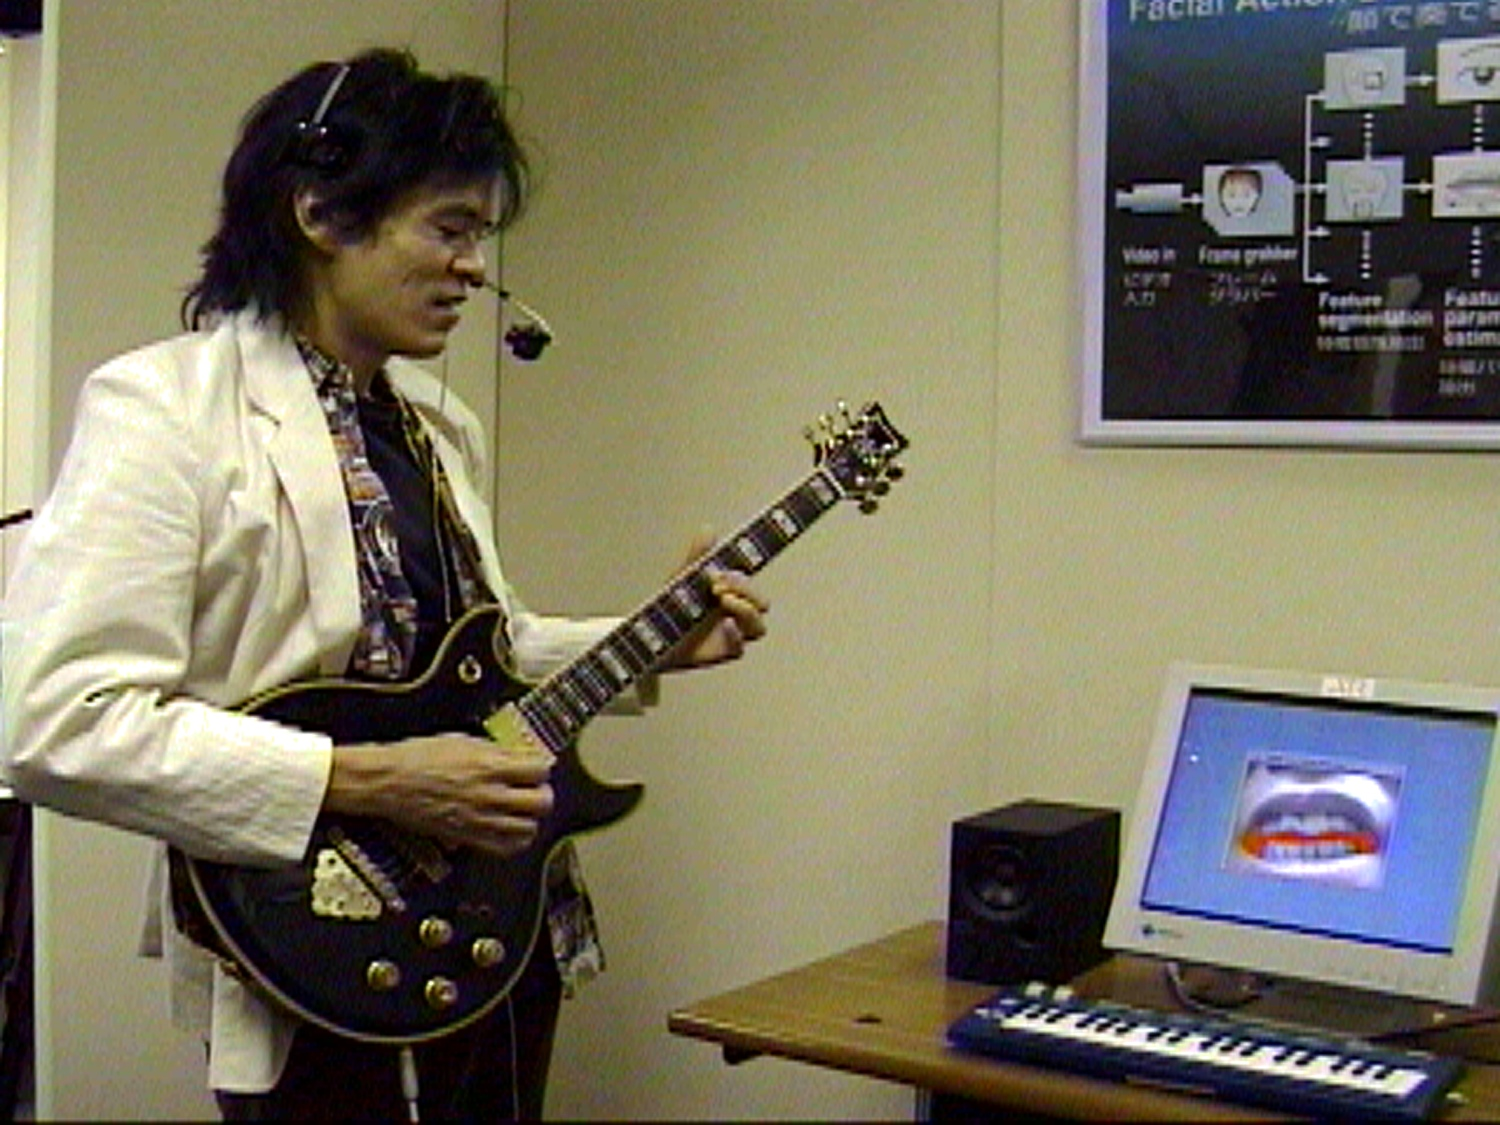
\includegraphics[width=\textwidth]{lyons_fig5}
\caption{Controlling guitar effects with the Mouthesizer.}
\label{lyons-fig:5} 
\end{figure}

Ichiro Umata, jazz guitarist and cognitive science researcher, used the Mouthesizer to control guitar effects (Figure~\ref{lyons-fig:5}). Mouth height controlled wah-wah as described above and mouth width adjusted the amount of distortion. This experiment used an early version of the Mouthesizer running at 15 fps on an SGI O2 computer. The guitarist had little prior practice using the Mouthesizer.  After a session lasting approximately one hour, he noted that the Mouthesizer was easily learned and more natural to play than a pedal controller.  He also observed that changes of mouth width and height are correlated for most movements, making the controller more interesting to use than if the two audio effects were independently adjustable. This agrees with the findings of Hunt et al. in their study of simple and complex mappings.

\subsubsection{Keyboard Synthesizer Demo}

We experimented with several keyboard synthesizer patches running on the Nord Modular, controlling patch parameters with the Mouthesizer. We tried these at a live demo during the ATR Open House exhibition. The mappings which easiest for most visitors to understand were simple ones usually associated with keyboard pedals such as volume control, sustain, and damping.

Reactions to the Mouthesizer varied greatly. Some visitors, having conservative musical tastes, found the concept strange or at least humourous. Others, sympathetic to electronic music, found it more appealing. 

\subsubsection{Sequenced Loops}

Inspired by the Augmented Groove system, we used the Mouthesizer to control techno loops. This allows one to add expression to an automatically played musical sequence. Again, sweeping filters, resonance, distortion, and formant filter morphs work well here.  

\section{Live Performance}
%\label{lyons-sec:5}

\begin{figure}[t]
\centering
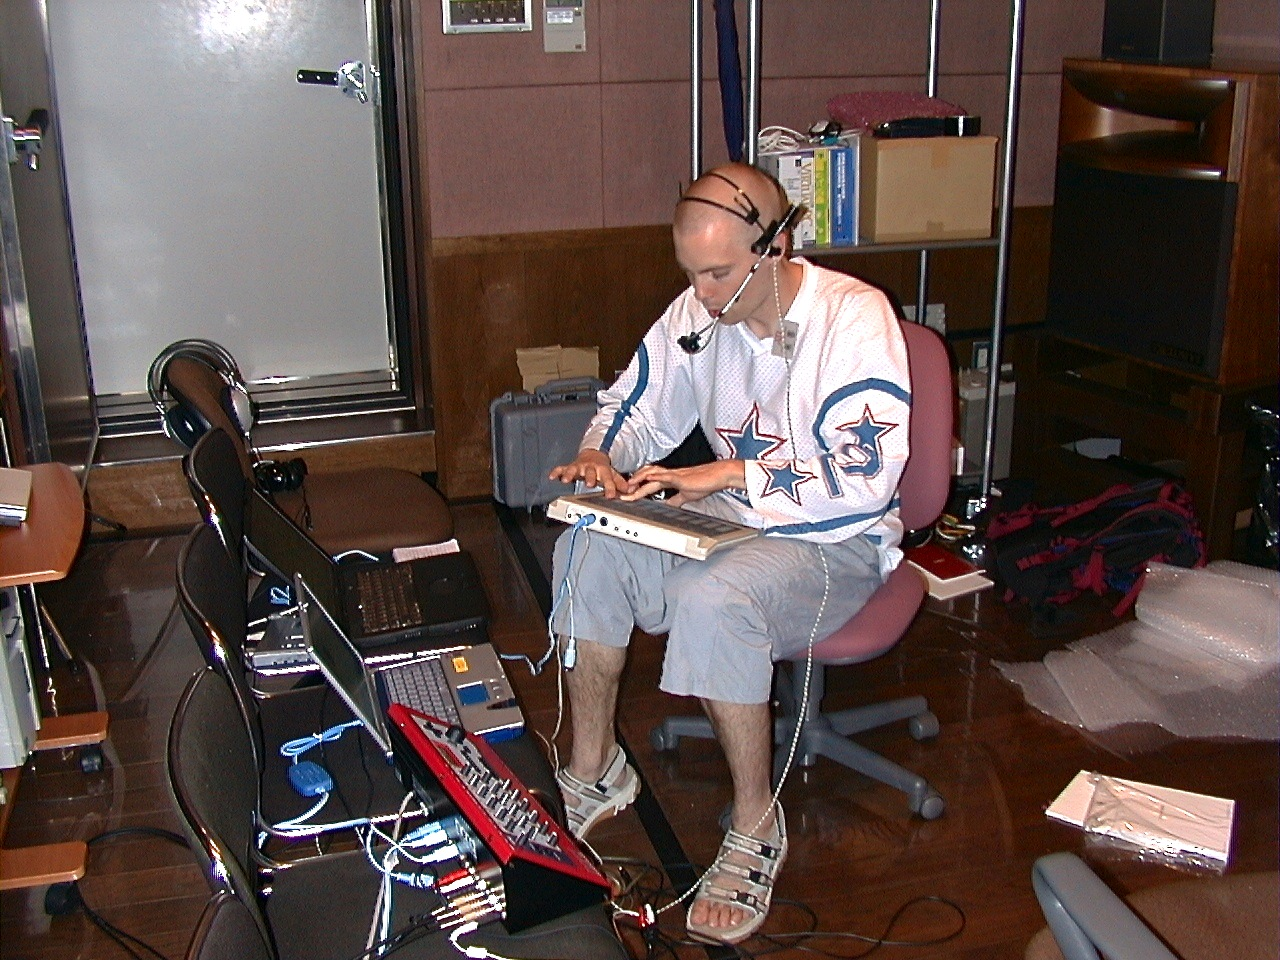
\includegraphics[width=\textwidth]{lyons_fig6}
\caption{Jordan Wynnychuk with controllers used for the live performance.}
\label{lyons-fig:6} 
\end{figure}

Jordan Wynnychuk gave a 30 minute solo live performance of improvised electroacoustic music using the Mouthesizer at the Kyoto Kyoryukan to audience of about 30 people. Figure~\ref{lyons-fig:6}), from our rehearsal for the performance, shows the instrumentation used in the concert. Jordan used a touch-sensitive MIDI control pad and STEIM's LiSa (Live Samples) software, to trigger and manipulate samples with the fingers of both hands. The sounds used in this performance consisted of glitches, squeaks, blips, bangs, buzzes, whirs, other “error” sounds, as well as samples of percussion instruments. 

Audio effects running on the Nord Modular were controlled using the Mouthesizer. Aesthetic considerations led us to experiment with audio effect mappings less intuitive than the ones described above, including a mix of extreme distortion, high and low pass. Figure~\ref{lyons-fig:7} shows a sequence of pictures from Jordan's performance in which a mouth gesture is being used to adjust sound expressively. Not visible in these images are the highlighted mouth shadow regions, which were projected on a screen beside the stage.

In addition to the interest and originality of Jordan's performance, audience members' attention seemed to be captured by the novelty of the Mouthesizer interface and concept. Many asked afterwards about how it worked or suggested ways it could be used to play music. One or two reported on their check for causality between mouth action and aural effect: they found it sometimes easily visible but quite obscure at other times. This appeared to be mainly a function of the mapping.

\section{Conclusion}
%\label{lyons-sec:6}

Experimentation with a variety of mappings and musical applications, and use of the Mouthesizer in a live public performance confirmed our hypothesis that facial gestures, especially movements of the mouth, are suitable for expressive musical control. Several lessons were learned in the design process.

Abandoning the head-tracking system early in the project later led us to avoid discrete classification of facial expressions for control of musical effects. This was fortunate: a controller which categorized emotion discretely would have limited responsiveness to movement quality and would reduce expressiveness. Rather, we captured a signal responsive to the motion of the mouth with a simple vision algorithm and relied on carefully chosen mappings to enable expressive control of sound production.

\begin{figure}[t]
\centering
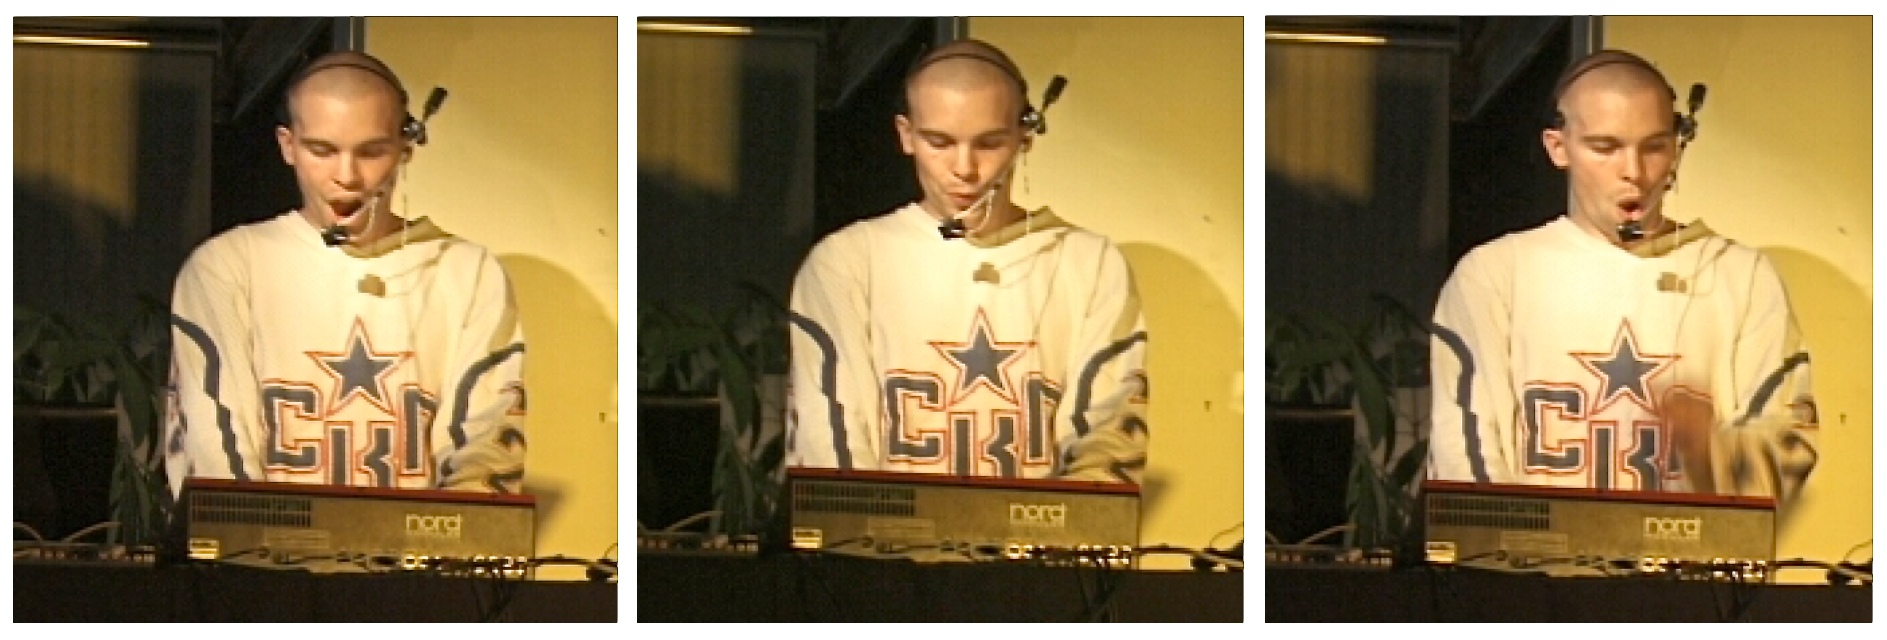
\includegraphics[width=\textwidth]{lyons_fig7}
\caption{Jordan Wynnychuk using the Mouthesizer in a live performance.}
\label{lyons-fig:7} 
\end{figure}

A valuable feature of the Mouthesizer is the visual feedback provided by highlighting segmented pixels. This gives a highly visible display mirroring the player's actions. Rizzolatti and colleagues \cite{Rizzolatti:1996} have discovered ``mirror neurons'' in monkey frontal lobes which respond to specific motor actions both when they are performed and when the same or a similar action is observed. Such circuits are thought to be important for learning motor behaviours. Controllers which mirror a motor action via visual display (and perhaps also auditory display?) should strongly stimulate these circuits. This may lend appeal to musical interfaces that mirror the player's gestures. A previous vision-based interface which shares this property is the Iamascope \cite{Fels:1999}. 

Additionally, visual perception of lip movement is known to affect auditory perception of speech \cite{McGurk:1976} (the “McGurk effect”). The Mouthesizer brings such cross-modal sensory mappings into play for both performer and observer. 

Such considerations lead us to conclude that video-based and other new gestural controllers offer much more than a visually engaging spectacle for the audience. They enable news ways to use the body and its sensory-motor systems to explore human expression and communication via sound. 

Recently the Mouthesizer was integrated with an improved face tracking system to create an interface which allows users to point and click with facial gestures. Hence, work on a musical interface led to a non-musical side product. Musical applications seem to stimulate exploration of a very wide range of interaction paradigms. In this way, the NIME conference may have an important contribution to make to the wider field of human-computer interaction. 

\begin{acknowledgement}
Thank you to Palle Dahlstedt, Sidney Fels, Steven Jones, Axel Mulder, Ivan Poupyrev, Ichiro Umata, Jordan Wynnychuk, and Tomoko Yonezawa for stimulating and helpful interactions.
\end{acknowledgement}


\section*{Author Commentary: Tales of the Mouthesizer---Facial Movements and Musical Expression}
\paragraph{Michael J. Lyons}

While working on automatic face recognition in the mid-nineties, I became interested in exploring facial movements in the context of real-time human computer interaction. This was partly in reaction to the dominant tendency of face recognition researchers to posit artificial agency as a primary research goal, implicitly defining the ideal \lq user\rq as a passive object surveilled by a machine. I was also influenced by the then emerging activity in embodied human computer interfaces which challenged the keyboard-mouse interaction style. A proposal to explore facial gesture interfaces was funded by the Annenberg Center at the University of Southern California. We recorded actors' facial movements,  detected and tracked facial features, and coded and analyzed local texture displacements using a biologically-inspired multi-scale Gabor filter representation. An unexpected and exciting discovery on facial expression representation led me to take a multi-year detour away from intentional gesture interfaces.

By mid-2000, I was again acutely feeling the limitations of the artificial agency paradigm tacit also in most facial expression research, I resumed work on the facial gesture interface project. Hoping to explore seamless, real-time, and actively expressive interaction I combined the project with my long-term interest in electronic music and began to develop a musical interface based on facial movements. I gradually reduced the complexity of our facial expression system, finally obtaining acceptable latency with a version which required the user to visually register their face with a virtual frame. The system was further simplified by analyzing just the shadow area of the open mouth, a fairly robust feature directly influenced by mouth movements. Adding a head-worn camera eliminated the need for active face registration. The Mouthesizer was born and, soon afterwards, was demonstrated as a guitar and keyboard effects controller at the annual ATR Labs Open House. 

A collaboration with artist Jordan Wynnychuk led to more complex mappings and the first public performance with the Mouthesizer. The experience encouraged us to continue the project. Jordan developed a new hardware prototype, the aluminum half-mask used in the NIME 2004 club performance  that Cornelius Poepel mentions in his commentary. A hand-held version was developed for a musical video game. Concurrently, I explored facial gesture interfaces in other contexts: text-entry, augmented digital painting, and a hands-free keyboard and cursor control system \cite{Chan:2008,Lyons:2004,Morikawa:2013}. The studies were not only exploratory, but involved measurements of controllability using custom evaluation tasks. To our surprise, single parameter control (mouth area) was observed possible with a signal-noise ratio exceeding 60dB \cite{Chan:2008,Morikawa:2013}!

We returned to expressive audio-visual play with a study of a mouth-activated bio-acoustic simulation \cite{Silva:2004}, that allowed a player to use mouth movements to sing like a bird---specifically a crow. Visiting research student Mathias Funk joined the facial gesture interface project and we collaborated on a biologically inspired system that combined a face detector, used to periodically saccade to the face, with optical flow estimation, allowing one to play a sampler by moving various facial features \cite{Funk:2005}. The work was demonstrated at NIME 2005, used in a live dance performances, and for special effects in a technology-augmented theatre production.

As sensor technologies and machine learning advance, we can expect to see powerful new approaches to gauge facial movements non-invasively. For example, the recent radar sensors from Project Soli\footnote{\url{https://www.google.com/atap/project-soli/}} may be suitable for use as a facial gesture interface. Close-range depth imaging also seems promising. Machine learning should be useful for leveraging existing expertise involved in facial expression and speech production, and should lead to intriguing new approaches to expressive performance, just as the Mouthesizer allowed us to map mouth movements to acoustic and emotionally expressive effects. The complex facial sensory-motor anatomy offers a still largely unexplored territory for scientific and artistic experiments in embodied musical expression. 

\section*{Expert Commentary: Musical Control and Musical Expression}
\paragraph{Cornelius Poepel}

As a musician I am focusing on the question of musical expression. I have long been interested to expand artistic expressivity through the use of technology and computation. During my visits to several NIME conferences the concerts were of high importance for me, especially those performances where I could hear and see the instruments in action that had been described in papers. 

I remember listening to a NIME club night concert in 2004 at Hamamatsu. A performer was playing the Mouthesizer \cite{Lyons:2003}. A camera tracking the mouth was mounted inside an aluminum  case which the performer had fixed in front of his mouth. A video screen displayed one window showing the video tracked mouth, another window showing an Ableton live set, and a third window showing artificial visual objects. In my subjective perception the whole setup resembled a mixture of Star Wars' Darth Vader, C-3PO, and Luke Skywalker. I loved to watch this performance following the varying shapes of the mouth while listening to linked variations in the resulting sound. 

The face and the facial gestures undeniably play a central role in communication. Music psychologists have shown that visual factors can play an important role in the perceived quality of musical expression \cite{Behne:2011}. One may say that the perceived musical expression is created not only by the acoustic outcome, it is created by a mixture of acoustic as well as other (e.g. visual) stimuli. 

Thus, the idea of using the expressivity we know from facial gestures has a powerful potential. The question is how this expressivity can be mapped to music, to the input parameters of a synthesis or an effects unit. 

Lyons et al. \cite{Lyons:2003} have blazed a trail with their work and a decade later papers still use this work for reference. The broad analysis of related research presented in their paper, the detailed explanation of the implementation of their idea, the incorporation of experiences coming from users and a live performance, laid a base that was and is valuable many years later, even now. 

From my point of view, I would say that the way in which to use the expressive power of facial gestures for musical expression is still an open question.  I was involved in the development of a singing voice synthesis installation that incorporated a mouth tracking system to control a voice synthesizer \cite{Poepel:2014}. Since the facial gestures drive a voice synthesizer, the resulting sounds corresponded to human expectations.

In comparison, the Mouthesizer as I saw it at the NIME 2004 club concert did not allow the display of the complete facial expression. Nose, mouth, cheek and chin were covered by the aluminum case mounted on the performer's face. Thus the visual part of the facial expressivity was reduced to the part one could see on the video screen. 

Dobrian and Koppelman have presented their thoughts and findings on the \lq E \rq in NIME \cite{Dobrian:2006}. They are convinced that control should not be equated with expression. They distinguish between control of a tool or medium and the expression a performer puts into the control mechanism of a sound generator. How can this conviction be of use in constructing a vision-based mouth-interface?

What kinds of expression come to my mind when I imagine faces? I see expressions like  sadness, happiness, anger, fear, effort etc. In the singing voice installation \cite{Poepel:2014} it was possible to play with facial gestures addressing those issues since the mouth tracking was used to generate the vowels. Pitch e.g. was controlled by the arms. Thus the facial gesture had a degree of freedom for visual expression that was not directly coupled to the sound. 

Thanks to Lyons et al. the exciting research-field of facial gestures and musical expression has been opened. The map has several blank regions for further exploration. Consider the following two possibilities. The first one is to explore how the already known forms of facial expression can be coupled to a music generator producing music corresponding with emotions and communicative contents. The second one is the question how many of the facial movements should not control the sound and should be left to freely communicate via facial expression with the audience in order to enhance the audio-visually perceived musical expression (cf. \cite{Behne:2011}). This incorporates the question which parts of the face should be kept visible when a performance with a vision-based mouth interface is done.
